\documentclass{beamer}

\usepackage[utf8]{inputenc}   % Підтримка UTF-8
\usepackage[ukrainian]{babel} % Підтримка української мови
\usepackage[ukrainian=nohyphenation]{hyphsubst}
\usepackage{booktabs}
\usepackage[T2A]{fontenc}      % Кодова таблиця для кирилиці
\usepackage{amsmath, amsfonts} % Для математики, якщо потрібно
\usepackage{hyperref}          % Для створення посилань
\usepackage{listings}          % Пакет для вставки коду
\usepackage{graphicx}
\usepackage{csvsimple}
\usepackage{parskip}
\usepackage{csquotes}
\usepackage{xcolor}
\usepackage{multicol} % Для багатостовпчикового тексту

\usepackage{tabularray}
\usepackage{float}
\usepackage{codehigh}
\usepackage[normalem]{ulem}

\UseTblrLibrary{booktabs}
\UseTblrLibrary{siunitx}
\newcommand{\tinytableTabularrayUnderline}[1]{\underline{#1}}
\newcommand{\tinytableTabularrayStrikeout}[1]{\sout{#1}}
\NewTableCommand{\tinytableDefineColor}[3]{\definecolor{#1}{#2}{#3}}

\usetheme{Madrid}

% Прибираєм навігацію з кожного слайду
\beamertemplatenavigationsymbolsempty

\title{Лабораторна робота №3}
\subtitle{Регресійний аналіз}
\subtitle{Команда №9}

% [], щоб прибрати імена з кожного слайду
\author[]{
  Баранівська В.О.,
  Корсун Є. В.,
  Хмарук О. Ю.,
  Літковський А.С.,
  Кудін Н. А.
}
\date{2025}

\begin{document}

\frame{\titlepage}

\graphicspath{{../../../}} % Ensure this path is correct or remove it if not needed

%Короткий підсумок ЛР 1-2 (якщо є свіжі погляди, можна ще зменшити/додати/змінити)

\begin{frame}
  \section{Набір даних}

  \frametitle{Зміст}
  \tableofcontents[currentsection]
\end{frame}

\begin{frame}
  \frametitle{Набір даних}

  Було вирішено дослідити якість повітря Тайваню. Уряд провінції намагається
  контролювати та покращувати якість повітря. Тому 17 грудня 2017 року була введена
  реформа \textit{Air Pollution Control Action Plan}.

  \begin{center}

  \end{center}
\end{frame}

% Подумав, що напевно в цей раз немає сенсу повторювати, те що було в 2 попередніх лабах
% \begin{frame}
%   \frametitle{Набір даних}
% 
%   Загальний опис датасету:
% 
%   \begin{enumerate}
%     \item Кількість рядків: 5\,882\,208
%     \item Кількість стовпців: 25
% 
%     \begin{itemize}
%       \item Числові: 19
%       \item Факторні: 4
%       \item Дата: 1
%       \item Інші: 1
%     \end{itemize}
%   \end{enumerate}
% \end{frame}

\begin{frame}
  \frametitle{Висновки EDA}
  \begin{itemize}
    \item Загальний рівень AQI по регіонам зменшується, тобто показники покращуються після початку реформи.
    Більш явні зміни очікувано помітні через декілька років після реформи.

    \item Якість повітря змінюється нерівномірно у містах.
  \end{itemize}
\end{frame}

% \begin{frame}
%   \frametitle{Висновки з гіпотез та довірчих інтервалів}
%   \begin{itemize}
%   \item 
%   \item 
% 
%   \end{itemize}
% \end{frame}

\begin{frame}
  \section{Мета дослідження}

  \frametitle{Зміст}
  \tableofcontents[currentsection]
\end{frame}

\begin{frame}
  \frametitle{Мета дослідження}
  Досліджуємо змінну AQI (індекс якості повітря):
  \begin{itemize}
    \item Як змінювалася після введення реформи
    \item Сезонні коливання протягом року
    \item Залежність від швидкості вітру
  \end{itemize}
\end{frame}

\begin{frame}
  \frametitle{Підготовка набору даних}

  Даний набір даних є панельним. Для аналізу будемо використовувати модель з фіксованими ефектами.

  \begin{itemize}
    \item Залежна змінна: AQI
    \item Незалежні змінні: reform\_days\footnotemark, july\_days\footnotemark, windspeed
    \item Контрольні змінні:  –
    \item Фіксовані ефекти: county
  \end{itemize}

  \footnotetext[1]{Різниця між датою вимірювання і \textit{17 грудня 2017 року}, порахована в днях}
  \footnotetext[2]{Кількість днів до найближчого 1 липня (найнижча медіана AQI за рік)}
\end{frame}

\begin{frame}
  \frametitle{Підготовка набору даних}

  Для спрощення моделювання перетворимо початковий датасет:
  
  \begin{itemize}
    \item Згрупуємо дані за датою (без часу)
    \item Знайдемо медіану в кожній групі в числових змінних
  \end{itemize}

  Таким чином, з набору даних на 5\,882\,208 рядків отримуємо 231\,863 рядків, що значно пришвидшує створення моделі.
\end{frame}

% \begin{frame}
%   \frametitle{Пропущені дані по змінним}
%    
% \end{frame}

\begin{frame}
  \section{Моделювання}
  
  \frametitle{Зміст}
  \tableofcontents[currentsection]
\end{frame}

\begin{frame}
  \frametitle{Гіпотези про коефіцієнти}

  Структурна модель:

   $$AQI \sim \beta_1 \, \text{reform\_days} + \beta_2 \, \text{july\_days} + \beta_3 \, \text{windspeed} + \alpha $$

  \begin{enumerate}
    \item $\beta_1$: Очікується \textbf{негативний знак}. 
    Метою реформи було покращення якості повітря,
    тому після її впровадження AQI мав би знизитися.

    \item $\beta_2$: Очікується \textbf{позитивний знак}. 
    Влітку AQI знижується, а в інші сезони підвищується.

    \item $\beta_3$: Очікується \textbf{негативний знак}. 
    Сильніший вітер зазвичай сприяє кращому розсіюванню забруднювачів, 
    що призводить до зниження AQI (покращення якості повітря).
  \end{enumerate}
\end{frame}

\begin{frame}
  \frametitle{Модель 1}

  Почнемо з простої моделі, поступово додаватимемо більше регресорів:

   $$AQI \sim \beta_1 \, \text{reform\_days} + \alpha $$

  Оцінка моделі:

  \begin{table}
  \centering
  \begin{talltblr}[         %% tabularray outer open
  entry=none,label=none,
  note{}={+ p \num{< 0.1}, * p \num{< 0.05}, ** p \num{< 0.01}, *** p \num{< 0.001}},
  ]                     %% tabularray outer close
  {                     %% tabularray inner open
  colspec={Q[]Q[]},
  column{2}={}{halign=c,},
  column{1}={}{halign=l,},
  hline{4}={1,2}{solid, black, 0.05em},
  }                     %% tabularray inner close
  \toprule
  & 1 \\ \midrule %% TinyTableHeader
  reform\_days & \num{-0.007474}*** \\
  & (\num{0.000879}) \\
  Num.Obs. & \num{231361} \\
  \bottomrule
  \end{talltblr}
  \end{table}
   
\end{frame}

\begin{frame}
  \frametitle{Перевірка моделі 1 на стійкість}
  
  \begin{itemize}
    \item Модель 1.1: $$AQI \sim \beta_1 \, \text{reform\_days} + \alpha $$
    \item Модель 1.2 (квадратичний поліном): $$AQI \sim \beta_1 \, \text{reform\_days} + \beta_2 \, \text{reform\_days}^2 + \alpha $$
    \item Модель 1.3 (логаритм): $$AQI \sim \beta_1 \, \log(\text{reform\_days}) + \alpha $$
  \end{itemize}
\end{frame}

\begin{frame}
  \frametitle{Перевірка моделі 1 на стійкість}
  
  Коефіцієнт біля ключового регресора залишається від'ємним:
   
  \begin{table}
  \centering
  \begin{talltblr}[         %% tabularray outer open
  entry=none,label=none,
  note{}={+ p \num{< 0.1}, * p \num{< 0.05}, ** p \num{< 0.01}, *** p \num{< 0.001}},
  ]                     %% tabularray outer close
  {                     %% tabularray inner open
  colspec={Q[]Q[]Q[]Q[]},
  column{2,3,4}={}{halign=c,},
  column{1}={}{halign=l,},
  hline{8}={1,2,3,4}{solid, black, 0.05em},
  }                     %% tabularray inner close
  \toprule
  & 1.1 & 1.2 & 1.3 \\ \midrule %% TinyTableHeader
  reform\_days & \num{-0.007474}*** & \num{-0.015273}*** &  \\
  & (\num{0.000879}) & (\num{0.001062}) &  \\
  I(reform\_days\textasciicircum{}2) &  & \num{0.000004}*** &  \\
  &  & (\num{0.000000}) &  \\
  I(log(reform\_days)) &  &  & \num{-5.586250}*** \\
  &  &  & (\num{0.758463}) \\
  Num.Obs. & \num{231361} & \num{231361} & \num{203888} \\
  \bottomrule
  \end{talltblr}
  \end{table}
\end{frame}

\begin{frame}
  \frametitle{Перевірка моделі 1 на стійкість}
  
  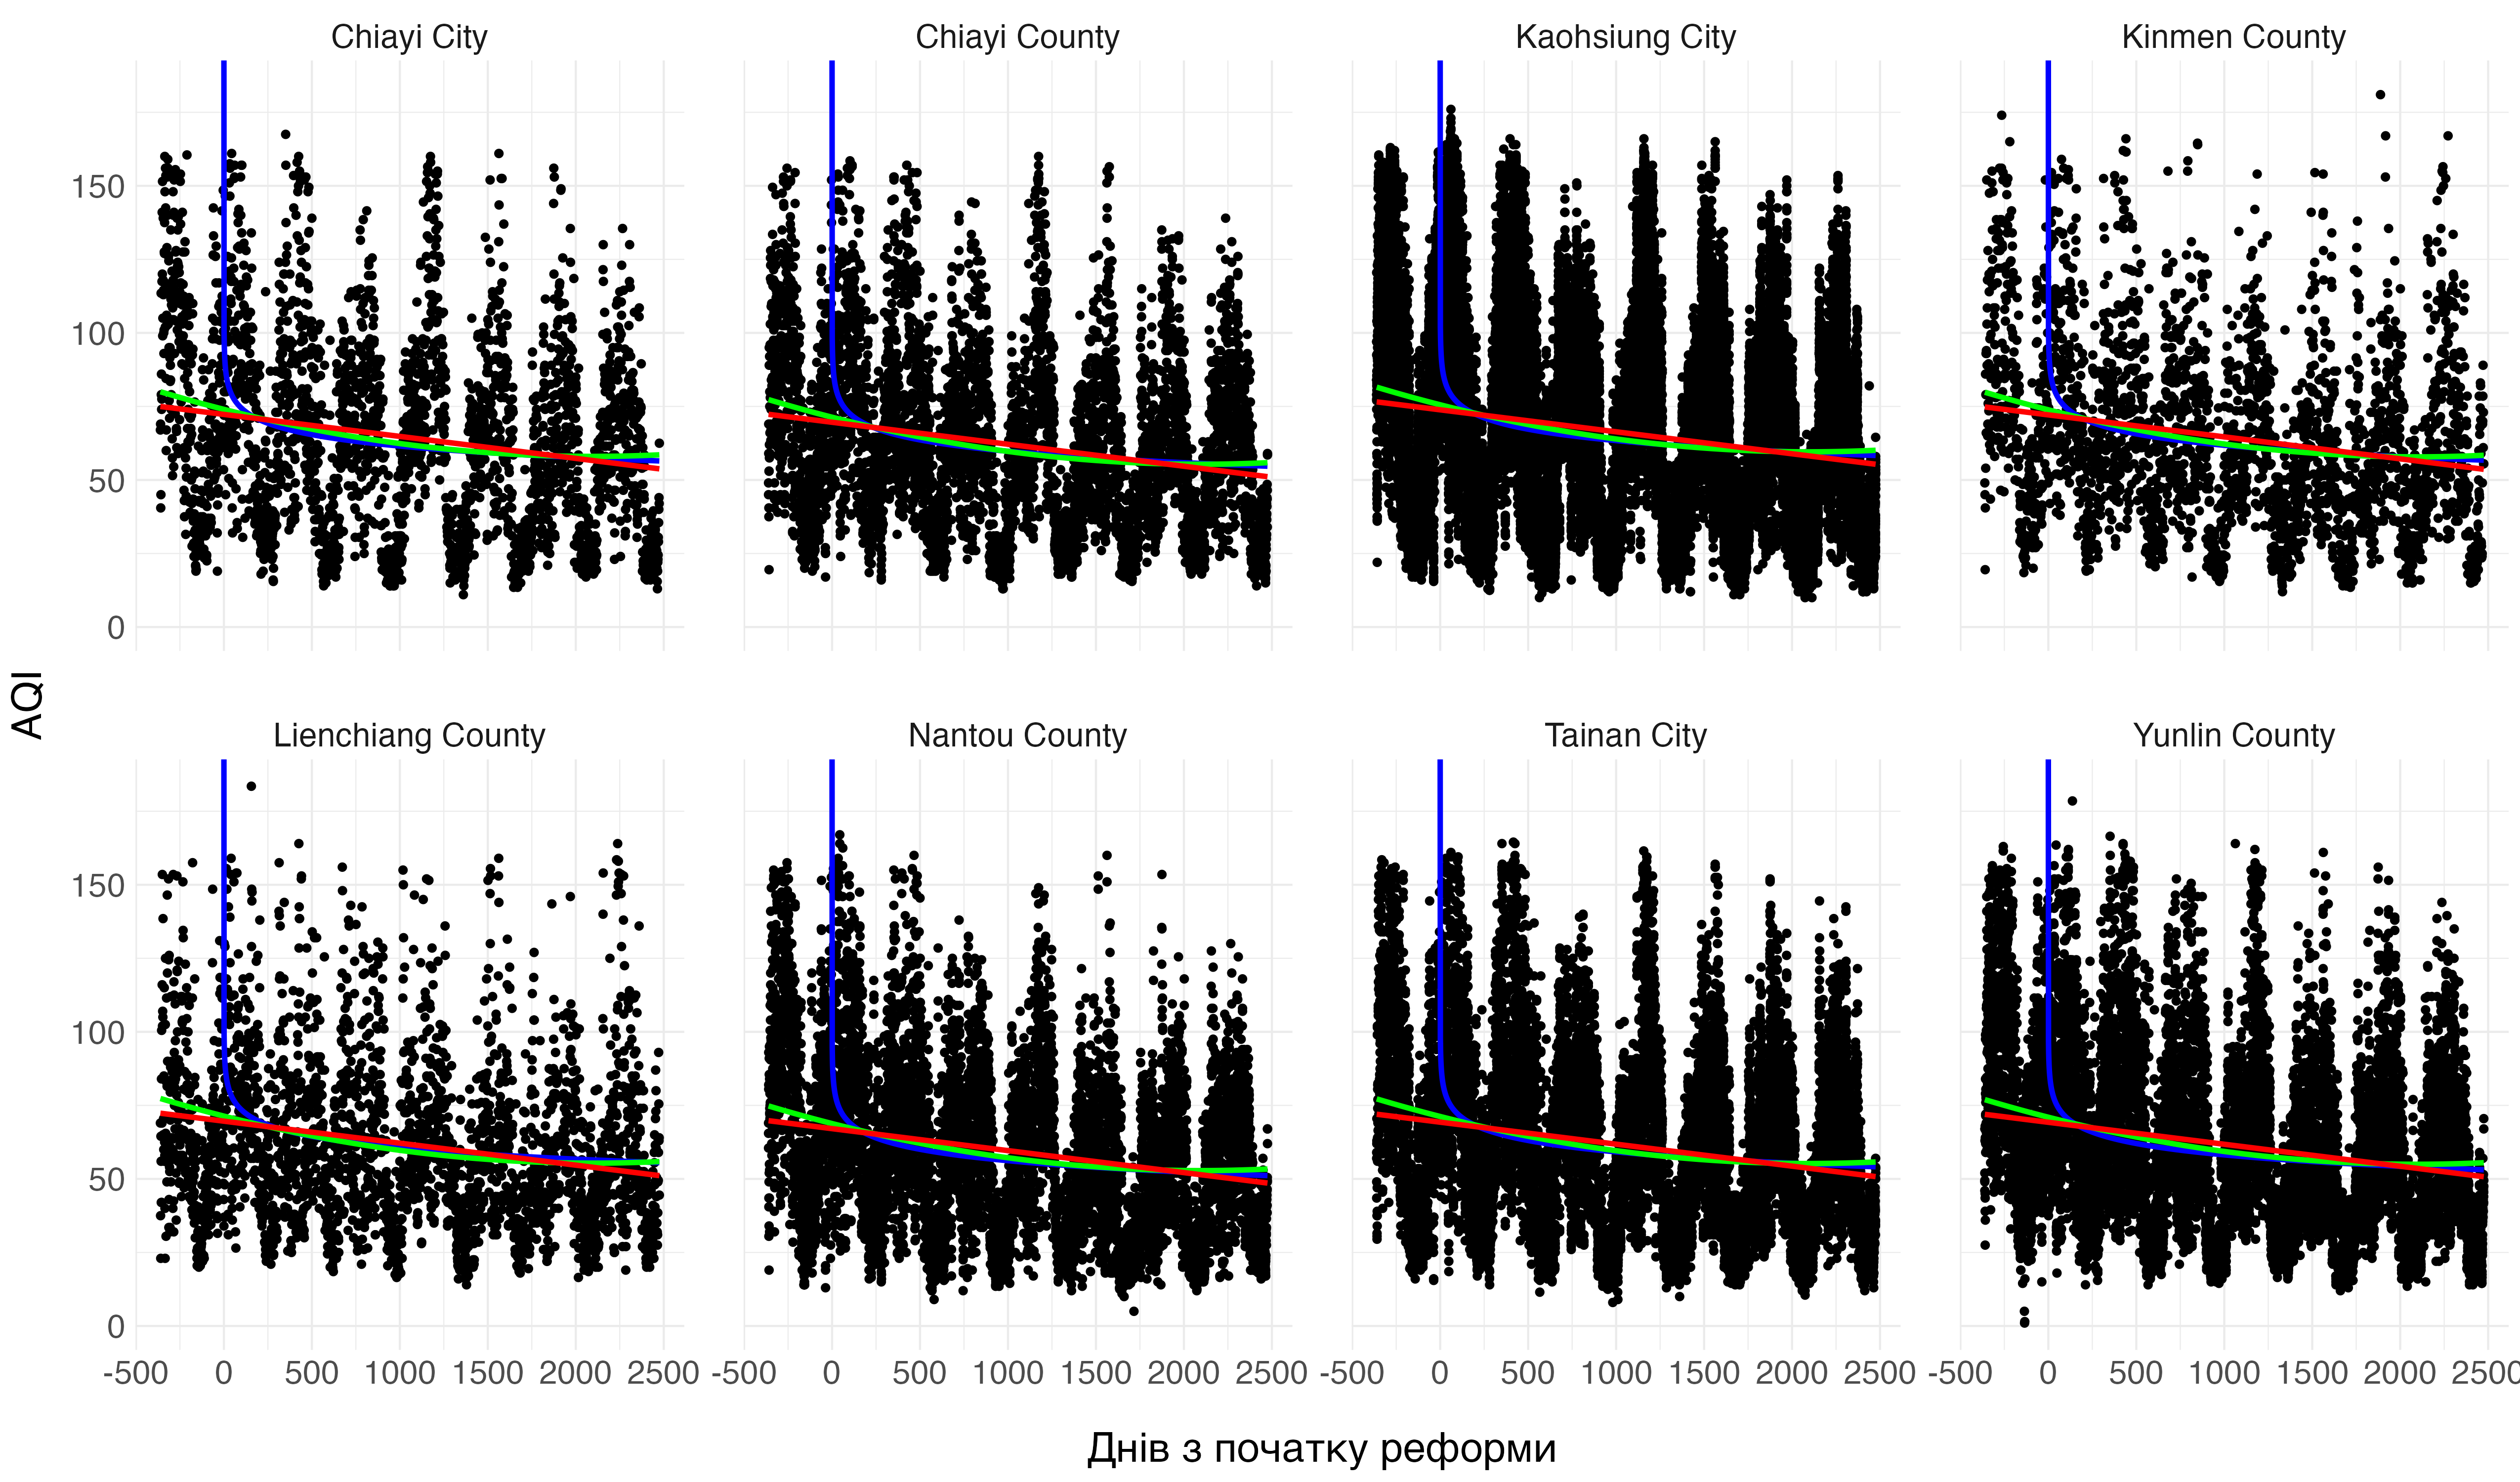
\includegraphics[height=2.8in]{plots/lab3/model-1-reform-vs-aqi.png}
\end{frame}

\begin{frame}
  \frametitle{Висновки по моделі 1}
  
  Отже:
  
  \begin{itemize}
    \item Залежність є від'ємною
    \item Всі коефіцієнти є статистично значущими
    \item Всі три версії моделі, починаючи з 250 днів близькі одна до одної
  \end{itemize}
  
  Робимо висновок, що початкова модель є стійкою відносно маніпуляцій з регресором reform\_days.
\end{frame}

\begin{frame}
  \frametitle{Модель 2}

  У ЛР 2 було підтверджено, що найменшу медіану AQI має в липні. Спробуємо додати змінну, що дорівнює кількості днів до найближчого липня. Розглянемо одразу випадки, коли регресор входить лінійно і у вигляді квадратичного поліному:

  \begin{itemize}
    \item Модель 2.1: $$AQI \sim \beta_1 \, \text{reform\_days} +  \beta_2 \, \text{july\_days} + \alpha $$
    \item Модель 2.2: $$AQI \sim \beta_1 \, \text{reform\_days} +  \beta_2 \, \text{july\_days} +  \beta_3 \, \text{july\_days}^2  + \alpha $$
  \end{itemize}
\end{frame}

\begin{frame}
  \frametitle{Оцінка моделі 2}
   
  \begin{table}
  \centering
  \begin{talltblr}[         %% tabularray outer open
  entry=none,label=none,
  note{}={+ p \num{< 0.1}, * p \num{< 0.05}, ** p \num{< 0.01}, *** p \num{< 0.001}},
  ]                     %% tabularray outer close
  {                     %% tabularray inner open
  colspec={Q[]Q[]Q[]},
  column{2,3}={}{halign=c,},
  column{1}={}{halign=l,},
  hline{8}={1,2,3}{solid, black, 0.05em},
  }                     %% tabularray inner close
  \toprule
  & 2.1 & 2.2 \\ \midrule %% TinyTableHeader
  reform\_days & \num{-0.006526}*** & \num{-0.006544}*** \\
  & (\num{0.000672}) & (\num{0.000674}) \\
  jul\_days & \num{0.193618}*** & \num{0.566284}*** \\
  & (\num{0.046703}) & (\num{0.050436}) \\
  I(jul\_days\textasciicircum{}2) &  & \num{-0.002038}*** \\
  &  & (\num{0.000148}) \\
  Num.Obs. & \num{231361} & \num{231361} \\
  \bottomrule
  \end{talltblr}
  \end{table}
\end{frame}

\begin{frame}
  \frametitle{Оцінка моделі 2}
  
  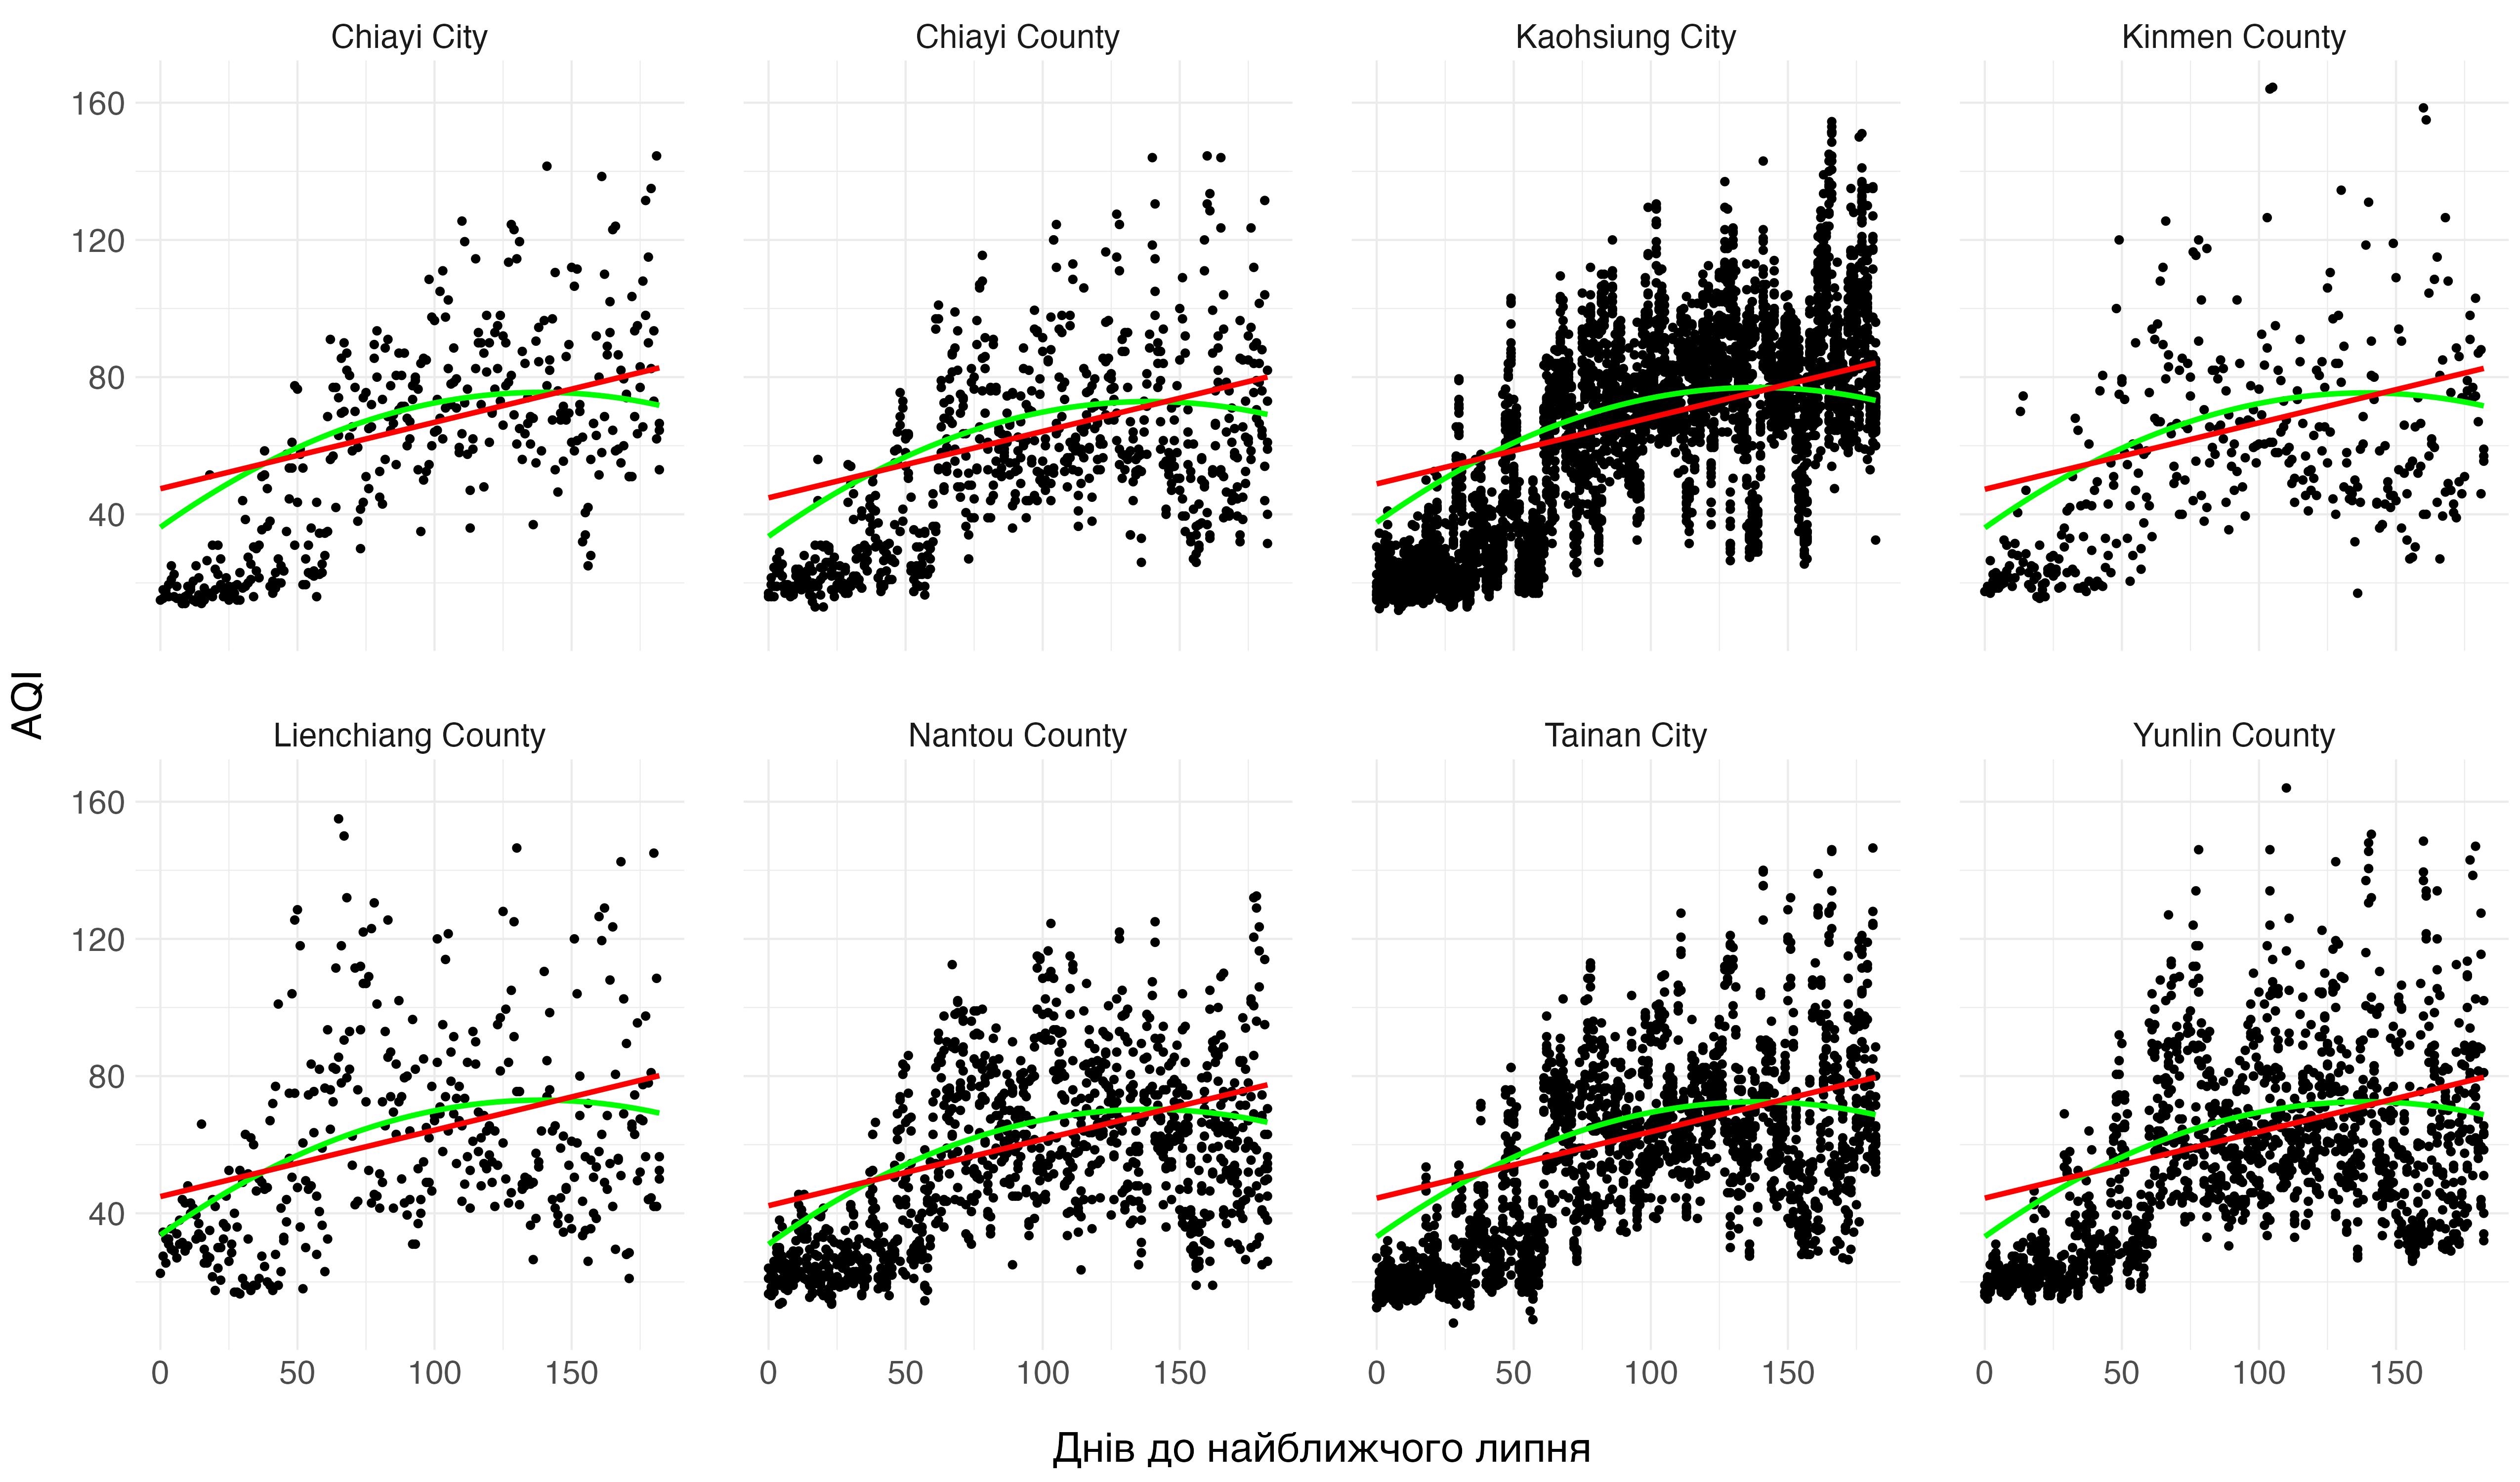
\includegraphics[height=2.8in]{plots/lab3/model-2-plus-jul_days-vs-aqi.png}
\end{frame}

\begin{frame}
  \frametitle{Оцінка моделі 2}
  
  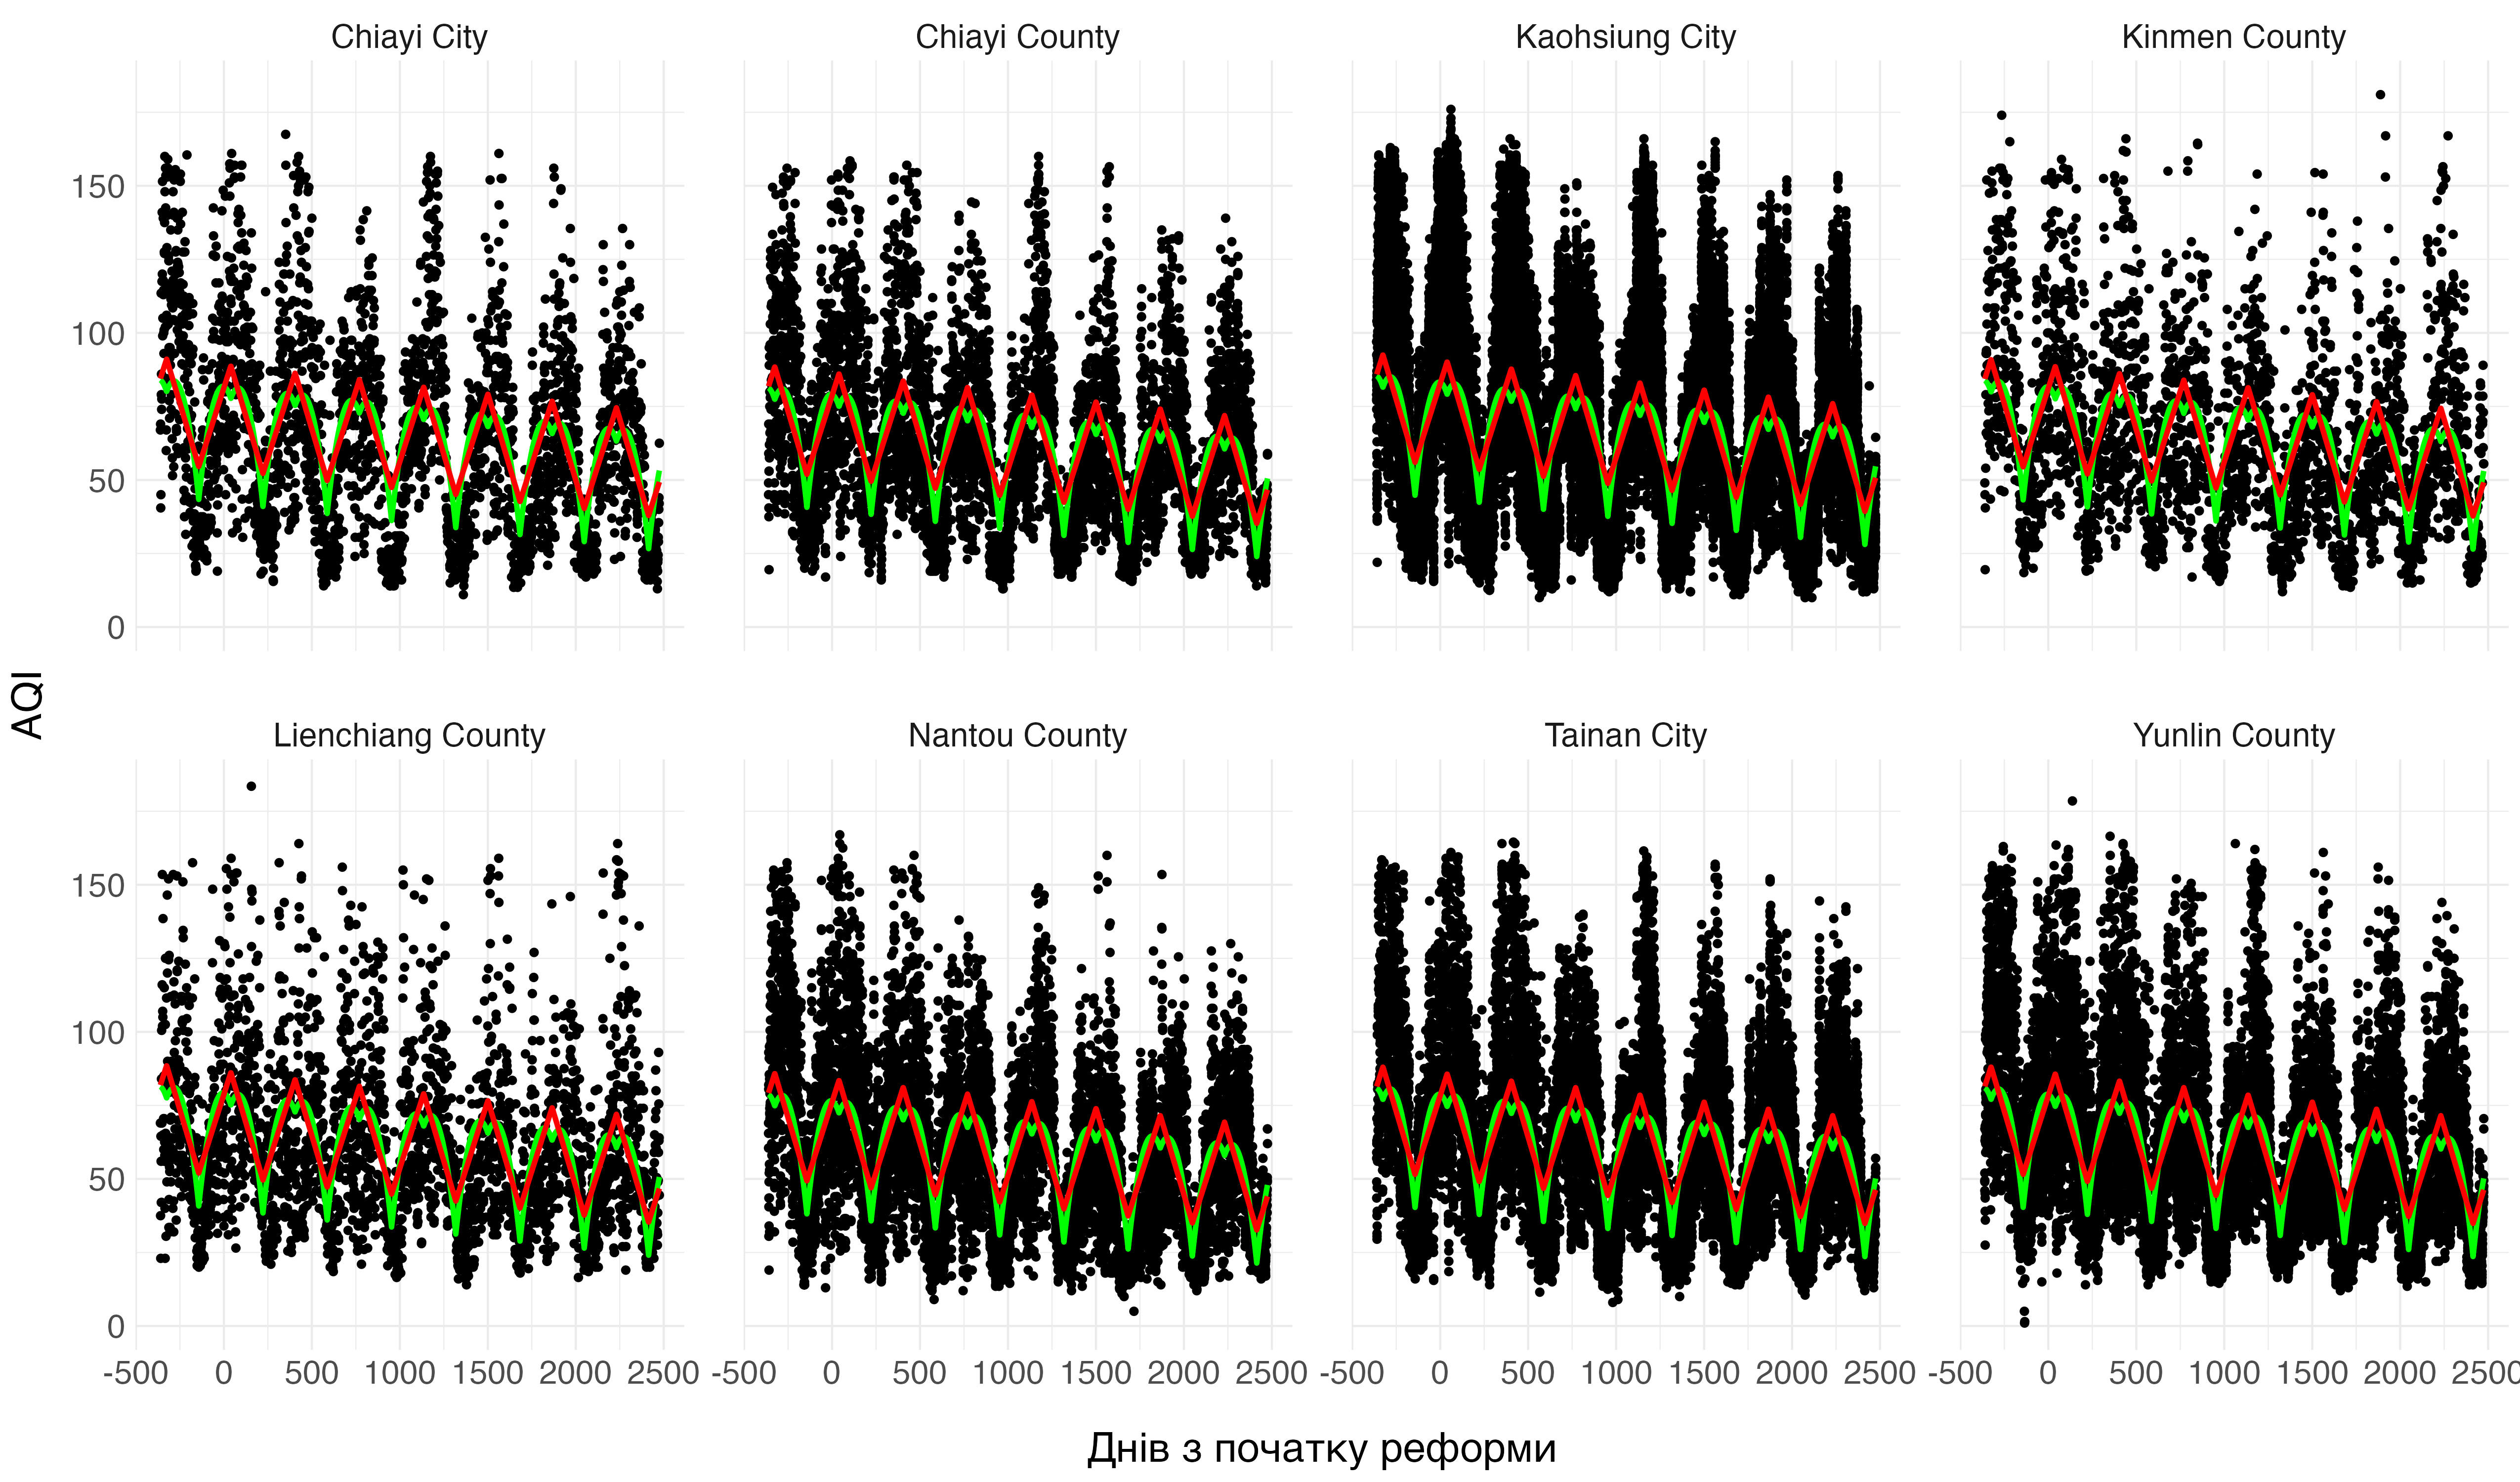
\includegraphics[height=2.8in]{plots/lab3/model-2-plus-reform-and-season-vs-aqi.png}
\end{frame}

\begin{frame}
  \frametitle{Висновки по моделі 2}
  
  Отже:
  
  \begin{itemize}
    \item Залежність є додатною
    \item Всі коефіцієнти є статистично значущими
    \item Регресор july\_days краще передає динаміку сезонних зміни у вигляді квадратичного поліному
  \end{itemize}
\end{frame}

\begin{frame}
  \frametitle{Модель 3}

  \begin{itemize}
    \item Модель 3.1:
    \begin{equation*}
      \begin{aligned}
        AQI & \sim \beta_1 \, \text{reform\_days} +  \beta_2 \, \text{july\_days} +  \beta_3 \, \text{july\_days}^2 +\\
               & + \beta_4 \, \text{windspeed} + \alpha
      \end{aligned}
    \end{equation*}
    \item Модель 3.2:
    \begin{equation*}
      \begin{aligned}
        AQI & \sim \beta_1 \, \text{reform\_days} +  \beta_2 \, \text{july\_days} +  \beta_3 \, \text{july\_days}^2 +\\
               & +  \beta_4 \, \text{windspeed} +  \beta_5 \, \text{windspeed}^2  + \alpha
      \end{aligned}
    \end{equation*}
    \item Модель 3.3:
    \begin{equation*}
      \begin{aligned}
        AQI & \sim \beta_1 \, \text{reform\_days} +  \beta_2 \, \text{july\_days} +  \beta_3 \, \text{july\_days}^2 +\\
               & + \beta_4 \, \log(\text{windspeed}) + \alpha
      \end{aligned}
    \end{equation*}
  \end{itemize}
\end{frame}

\begin{frame}
  \frametitle{Оцінка моделі 3}
   
  \begin{table}
  \centering
  \begin{talltblr}[         %% tabularray outer open
  entry=none,label=none,
  note{}={+ p \num{< 0.1}, * p \num{< 0.05}, ** p \num{< 0.01}, *** p \num{< 0.001}},
  ]                     %% tabularray outer close
  {                     %% tabularray inner open
  colspec={Q[]Q[]Q[]Q[]},
  column{2,3,4}={}{halign=c,},
  column{1}={}{halign=l,},
  hline{14}={1,2,3,4}{solid, black, 0.05em},
  }                     %% tabularray inner close
  \toprule
  & 3.1 & 3.2 & 3.3 \\ \midrule %% TinyTableHeader
  reform\_days & \num{-0.007285}*** & \num{-0.007511}*** & \num{-0.007590}*** \\
  & (\num{0.000663}) & (\num{0.000616}) & (\num{0.000634}) \\
  jul\_days & \num{0.578095}*** & \num{0.576953}*** & \num{0.575900}*** \\
  & (\num{0.046690}) & (\num{0.046161}) & (\num{0.045644}) \\
  I(jul\_days\textasciicircum{}2) & \num{-0.002009}*** & \num{-0.002001}*** & \num{-0.002010}*** \\
  & (\num{0.000143}) & (\num{0.000141}) & (\num{0.000141}) \\
  windspeed & \num{-2.550670}** & \num{-5.154686}*** &  \\
  & (\num{0.694160}) & (\num{0.789519}) &  \\
  I(windspeed\textasciicircum{}2) &  & \num{0.323383}** &  \\
  &  & (\num{0.090437}) &  \\
  I(log(windspeed)) &  &  & \num{-5.973826}*** \\
  &  &  & (\num{1.291077}) \\
  Num.Obs. & \num{221581} & \num{221581} & \num{221342} \\
  \bottomrule
  \end{talltblr}
  \end{table}
\end{frame}

\begin{frame}
  \frametitle{Оцінка моделі 3}
  
  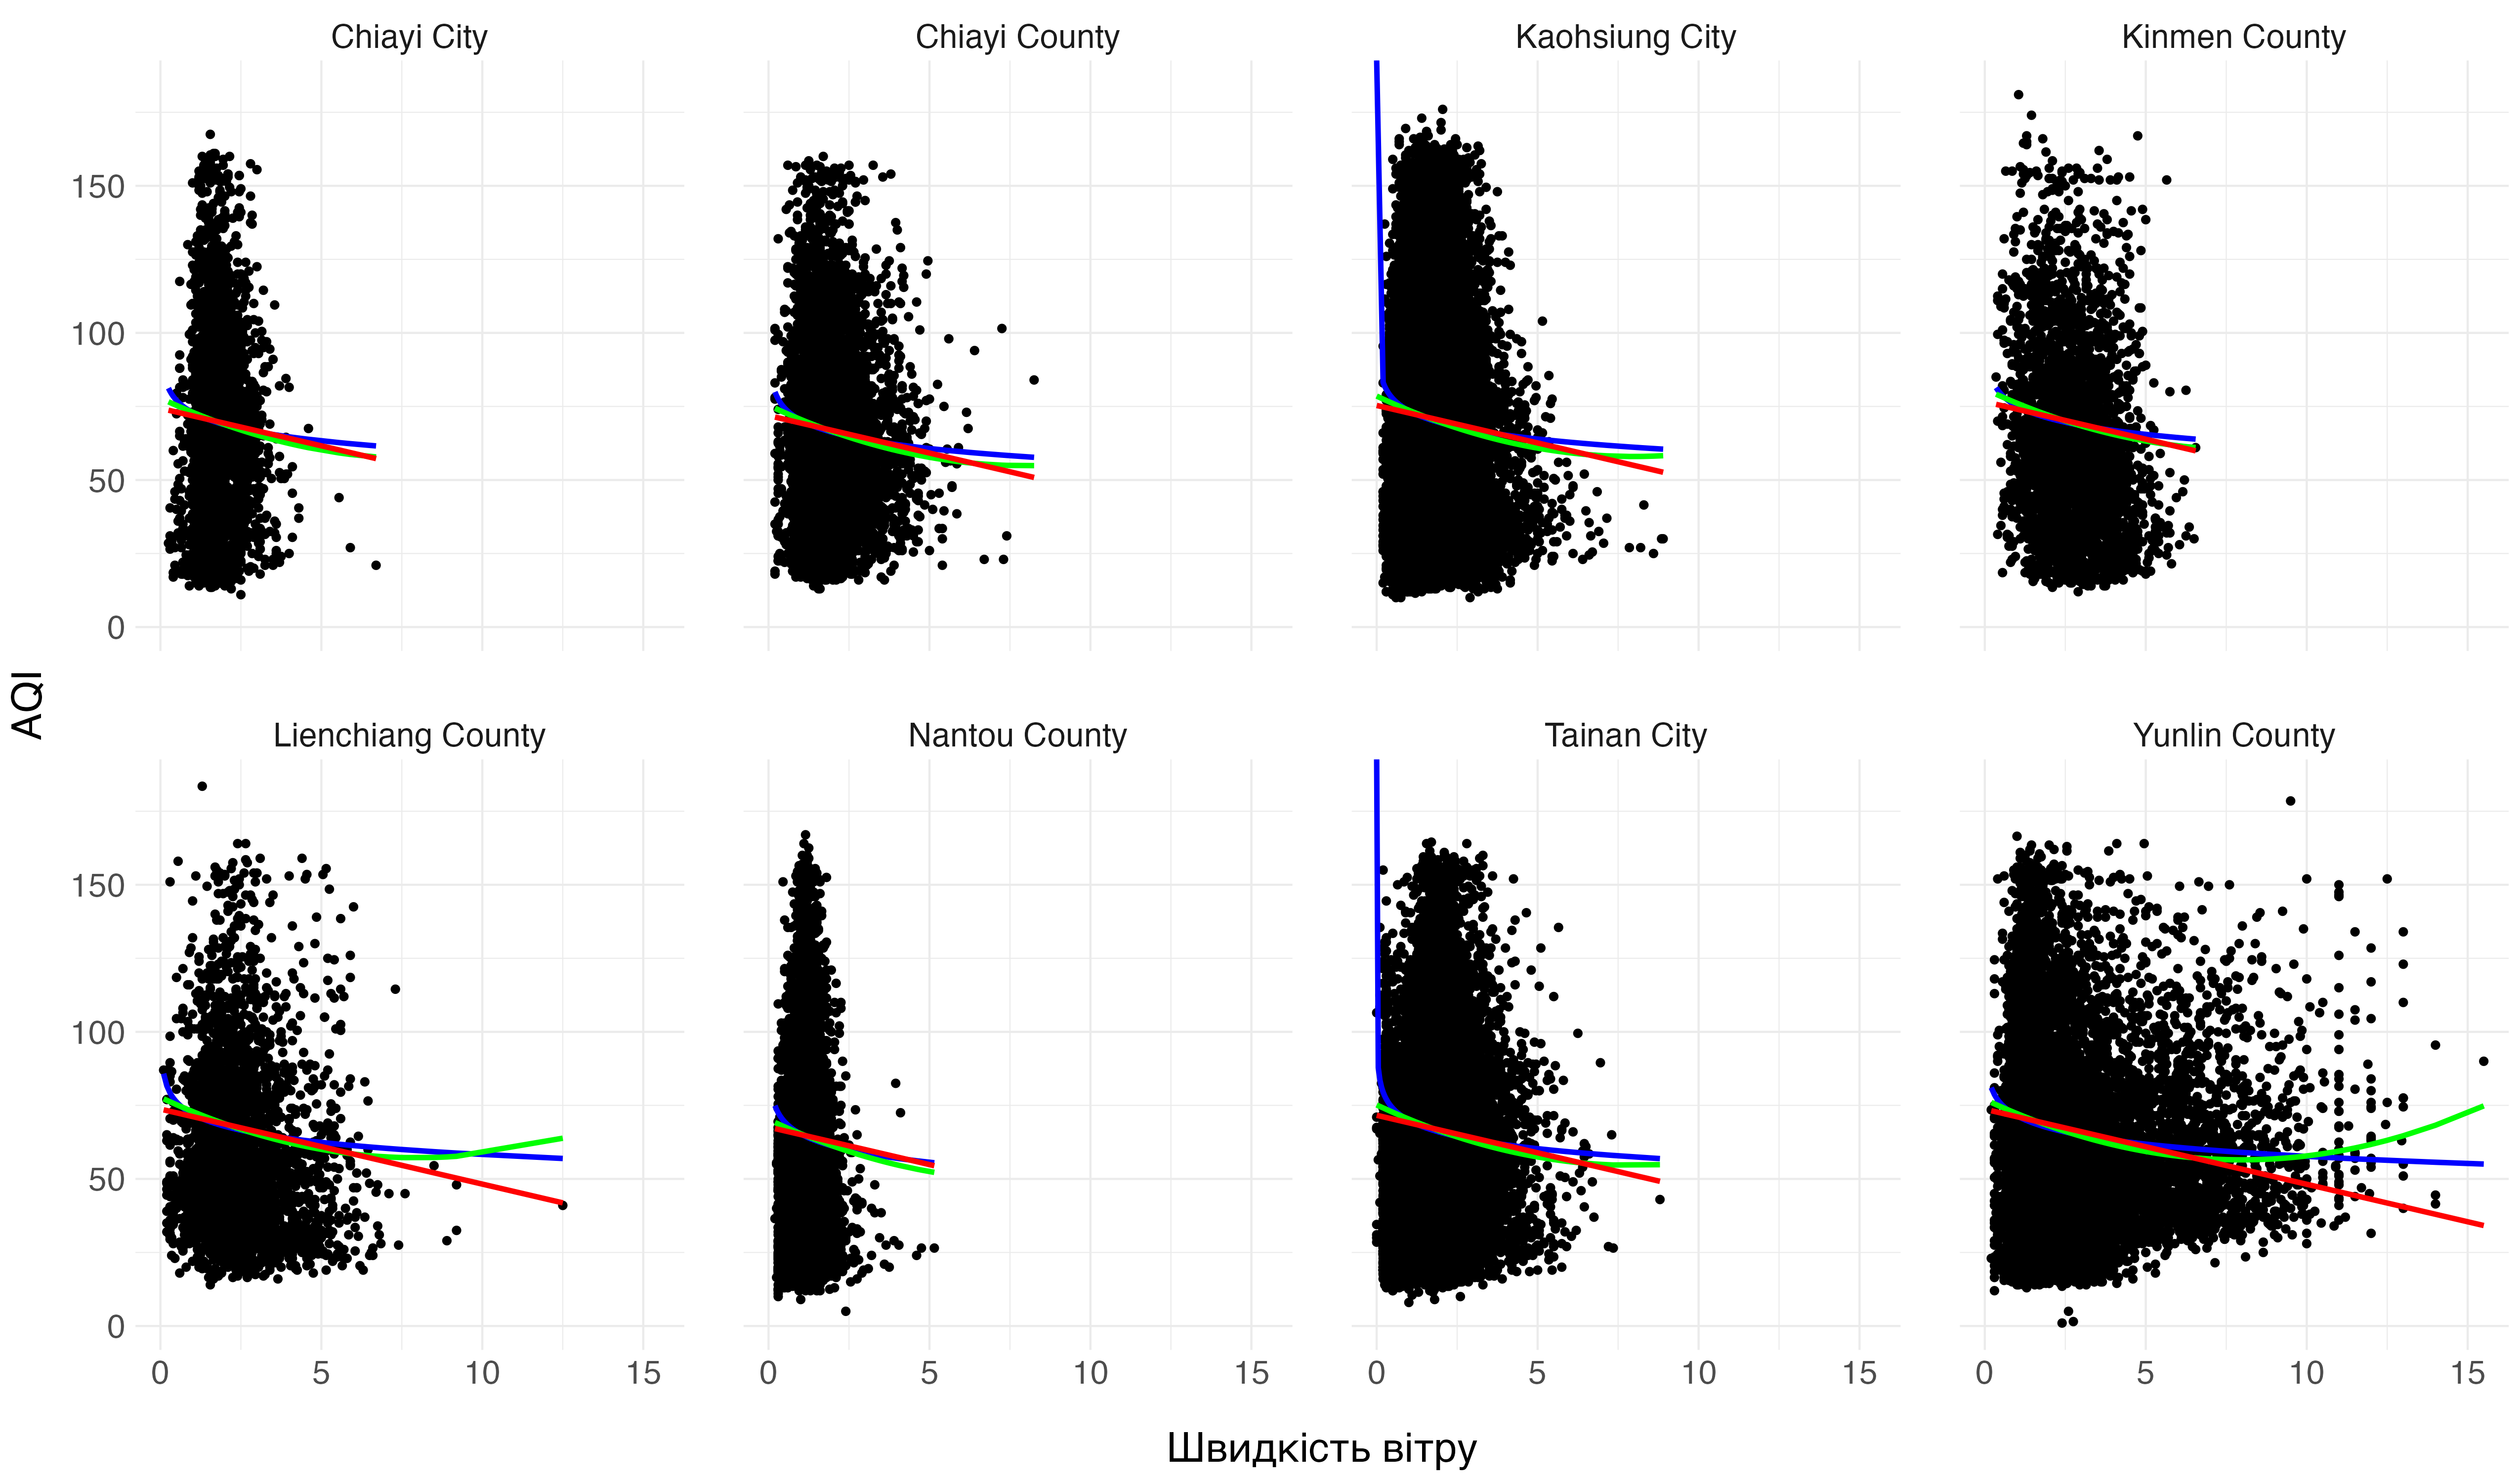
\includegraphics[height=2.8in]{plots/lab3/model-3-windspeed-vs-aqi.png}
\end{frame}

\begin{frame}
  \frametitle{Висновки по моделі 3}
  
  Отже:
  
  \begin{itemize}
    \item Залежність є від'ємною
    \item Всі коефіцієнти є статистично значущими
    \item Всі три версії моделі, до 10 м/с близькі одна до одної
  \end{itemize}
\end{frame}

\begin{frame}
  \frametitle{Коментар щодо стабільності}
  
  Під час додавання нових регресорів, поліномів вищих порядків відносно регресорів і взяття логарифмів змінних, коефіцієнт біля:
   
  \begin{itemize}
    \item $reform\_days$ коливався навколо -0.007474 в межах 0.001
    \item $jul\_days$ коливався навколо 0.566284 в межах 0.02
    \item $jul\_days^2$ коливався навколо -0.002038 в межах 0.00005
  \end{itemize}
  
  Тому модель можна вважати стійкою.
\end{frame}

\begin{frame}
  \frametitle{Коментар щодо стабільності}
   
  \begin{table}
  \centering
  \begin{talltblr}[         %% tabularray outer open
  entry=none,label=none,
  note{}={+ p \num{< 0.1}, * p \num{< 0.05}, ** p \num{< 0.01}, *** p \num{< 0.001}},
  ]                     %% tabularray outer close
  {                     %% tabularray inner open
  colspec={Q[]Q[]Q[]Q[]},
  column{2,3,4}={}{halign=c,},
  column{1}={}{halign=l,},
  hline{10}={1,2,3,4}{solid, black, 0.05em},
  }                     %% tabularray inner close
  \toprule
  & 1 & 2 & 3 \\ \midrule %% TinyTableHeader
  reform\_days & \num{-0.007474}*** & \num{-0.006544}*** & \num{-0.007285}*** \\
  & (\num{0.000879}) & (\num{0.000674}) & (\num{0.000663}) \\
  jul\_days &  & \num{0.566284}*** & \num{0.578095}*** \\
  &  & (\num{0.050436}) & (\num{0.046690}) \\
  I(jul\_days\textasciicircum{}2) &  & \num{-0.002038}*** & \num{-0.002009}*** \\
  &  & (\num{0.000148}) & (\num{0.000143}) \\
  windspeed &  &  & \num{-2.550670}** \\
  &  &  & (\num{0.694160}) \\
  Num.Obs. & \num{231361} & \num{231361} & \num{221581} \\
  \bottomrule
  \end{talltblr}
  \end{table}
\end{frame}

\begin{frame}
  \section{Висновок}

  \frametitle{Зміст}
  \tableofcontents[currentsection]
\end{frame}

\begin{frame}
  \frametitle{Висновок}
  
  В ході аналізу ми визначили, що:
  
   \begin{itemize}
    \item Після введення реформи рівень AQI з кожним днем зменшується на 0.007
    \item Є сезонні коливання AQI, хоча в датасеті немає даних, щоб дослідити, з чим саме це пов'язано
    \item Присутній від'ємний зв'язок між рівнем AQI і швидкістю вітру.
  \end{itemize}
\end{frame}
\end{document}